\documentclass{article}
\usepackage{graphicx}

\begin{document}

\section{Outlook}
% Description in report: Finally, an outlook will be given regarding the possible improvements in the future and the strategy to achieve these improvements. 

%introduction
\subsection*{Refactoring: Group 1}
We see many possibility's and improvements for in the future. Not for the reason that what we did was bad, but we believe that we made a start, a begin, to take back the control and overview of the project while even give the options for extending the BW4T. 

\subsection*{Possibility's}
Please take a look at the image below. This is an image taken of sonar which shows certain metrics of the BW4T-code. We will explain some improvements based on this. 
\begin{itemize}
	\item Testing: We started off course with 0,0\% test code and have now reached a 50,4\% coverage. While this is a great step forward, there are still a lot of classes/methods untested or test are not complete. Sometimes it was impossible for us to check a complete class. This had 2 reasons. 1: To complex to create a complete \emph{environment} to test a simple method. 2: PowerMocking was not possible.

\subparagraph*{PowerMocking}is a systems that enables testing of static/ final/private methods. It's a extension of \emph{Mockito} that uses previous versions of \emph{java}. While we use the newest version we aren't able to use PowerMocks. This makes it impossible to test many code. 

	\item Issues \& Technical Debt: At this moment there are 815 issues and we have a debt of 42 days. This is a lot and sometimes it's questionable if you should fix all the issues to lower the debt. 
	
	\item Decoupling: There are still to many dependencies in the project. There are 37 between packages and 96 between files. This also results in a Package tangle index of	27,6\%  (83 cycles).  
	
\end{itemize}
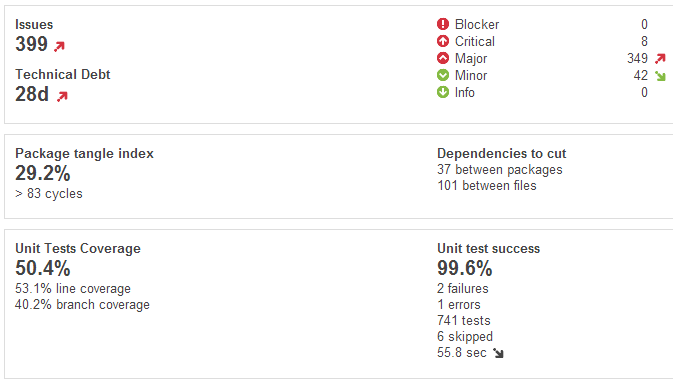
\includegraphics[scale=0.5]{statistics_group1}
	
\subsection*{Strategy}
\begin{itemize}
	\item Testing: Start with looking for a way to create an simple \emph{environment} to test the big classes like \emph{server} and \emph{client}. Also try to get PowerMock running (by waiting until it's becomes compatible, or finding another method). Make sure to continue testing! 
	\item Issues \& Technical Debt: Issues or divided in Blocker, Critical, Major, Minor and Info. Make sure there're no Blocker and Critical issues and took at least a look at the Major ones. This way you'll waste not to much time fixing issues compared to extending the code.  
	\item Decoupling: With \emph{Sonar} and \emph{Stan} you can visualize the dependencies. When you have an overview you can decide whether to change the class/package and try to cut dependencies. Sometimes restructuring will be needed. 
\end{itemize}



\end{document}
	